\documentclass{article}

\usepackage[utf8]{inputenc}
\usepackage[T1]{fontenc}
\usepackage{lipsum}
\usepackage{graphicx}
\usepackage{amsmath}
\usepackage[margin=1in]{geometry}
\usepackage{titlesec}
\usepackage{parskip}
\usepackage{tcolorbox}

\titleformat{\section}
{\LARGE\bfseries}{\thesection}{1em}{}

\titleformat{\subsection}
{\Large\bfseries}{\thesection}{1em}{}

\begin{document}

\pagestyle{empty}

\section*{Monadi}
\large

Una delle caratteristiche principali di Haskell è l'essere un linguaggio \textbf{lazy}.

Questa caratteristica porta ad alcune conseguenze positive, come:
\begin{itemize}
    \item Purezza: in un linguaggio completamente puro è presente la \textbf{trasparenza referenziale}.
    
    La trasparenza referenziale si può definire come: 
    
    \begin{center}
        Se \texttt{a = b} posso usare \texttt{a} al posto di \texttt{b} e viceversa.
    \end{center}

    Un possibile esempio di questo concetto può essere:
\begin{tcolorbox}
\begin{verbatim}
f x = a + a
    where
        a = g x
        b = h 3
\end{verbatim}
\end{tcolorbox}

    il quale viene tradotto dal compilatore Haskell in:
\begin{tcolorbox}
\begin{verbatim}
f x = g x + g x
\end{verbatim}
\end{tcolorbox}

    E' quindi possibile osservare come \texttt{a} venga sostituita con la sua definizione sottostante (ottimizzazione, \textbf{inlining}), andando a rimuovere completamente la definizione di \texttt{b} (non utilizzata).

    Questo è possibile solo se il linguaggio è puro, dove non è possibile alterare lo stato esterno.

    Se il linguaggio non fosse stato puro, \texttt{g} ed \texttt{h} avrebbero potuto causare effetti collaterali con la loro esecuzione. In questo caso, la traduzione effettuata dal compilatore non sarebbe stata corretta.
    \item Modularità dei programmi: è possibile dividere il programma in moduli differenti, richiamati solo se strettamente necessario.
    \item Normalizzazione (ad esempio, nel caso della funzione \texttt{const 1 undefined}, dove \texttt{undefined} non verrà mai valutato perché non utilizzato).
    \item Parallelismo: nei linguaggi pigri, e di conseguenza puri, è semplice parallelizzare l'esecuzione.
\end{itemize}
ma anche conseguenze negative, come:
\begin{itemize}
    \item Purezza: in un linguaggio completamente puro non è possibile stampare a schermo, stabilire connessioni di rete, ecc. Questo rende il linguaggio abbastanza inutile.
    \item Imprevedibilità: ad esempio, nel caso della funzione \texttt{const (print 1) (print 2)}, non si riesce a capire guardando solamente il codice quale sarà l'esito dell'esecuzione.
\end{itemize}

Un possibile esempio di purezza come conseguenza negativa in Haskell è la gestione di Input/Output (dialoghi). Prima delle monadi, questo procedimento richiedeva una logica contorta.

\pagebreak

Prima di introdurre il concetto di \textbf{monade}, bisogna fare una distinzione tra il \textit{fare qualcosa} rispetto al \textit{pensare di fare qualcosa}.

Nella programmazione tradizionale viene scritto in maniera esplicita quello che il programma deve fare, passo dopo passo.

Nella programmazione con monadi, il progrmama \textbf{crea delle azioni che se eseguite hanno un effetto collaterale} (come una stampa a schermo).

Una possibile rappresentazione grafica di questo concetto può essere:\\
\begin{center}
    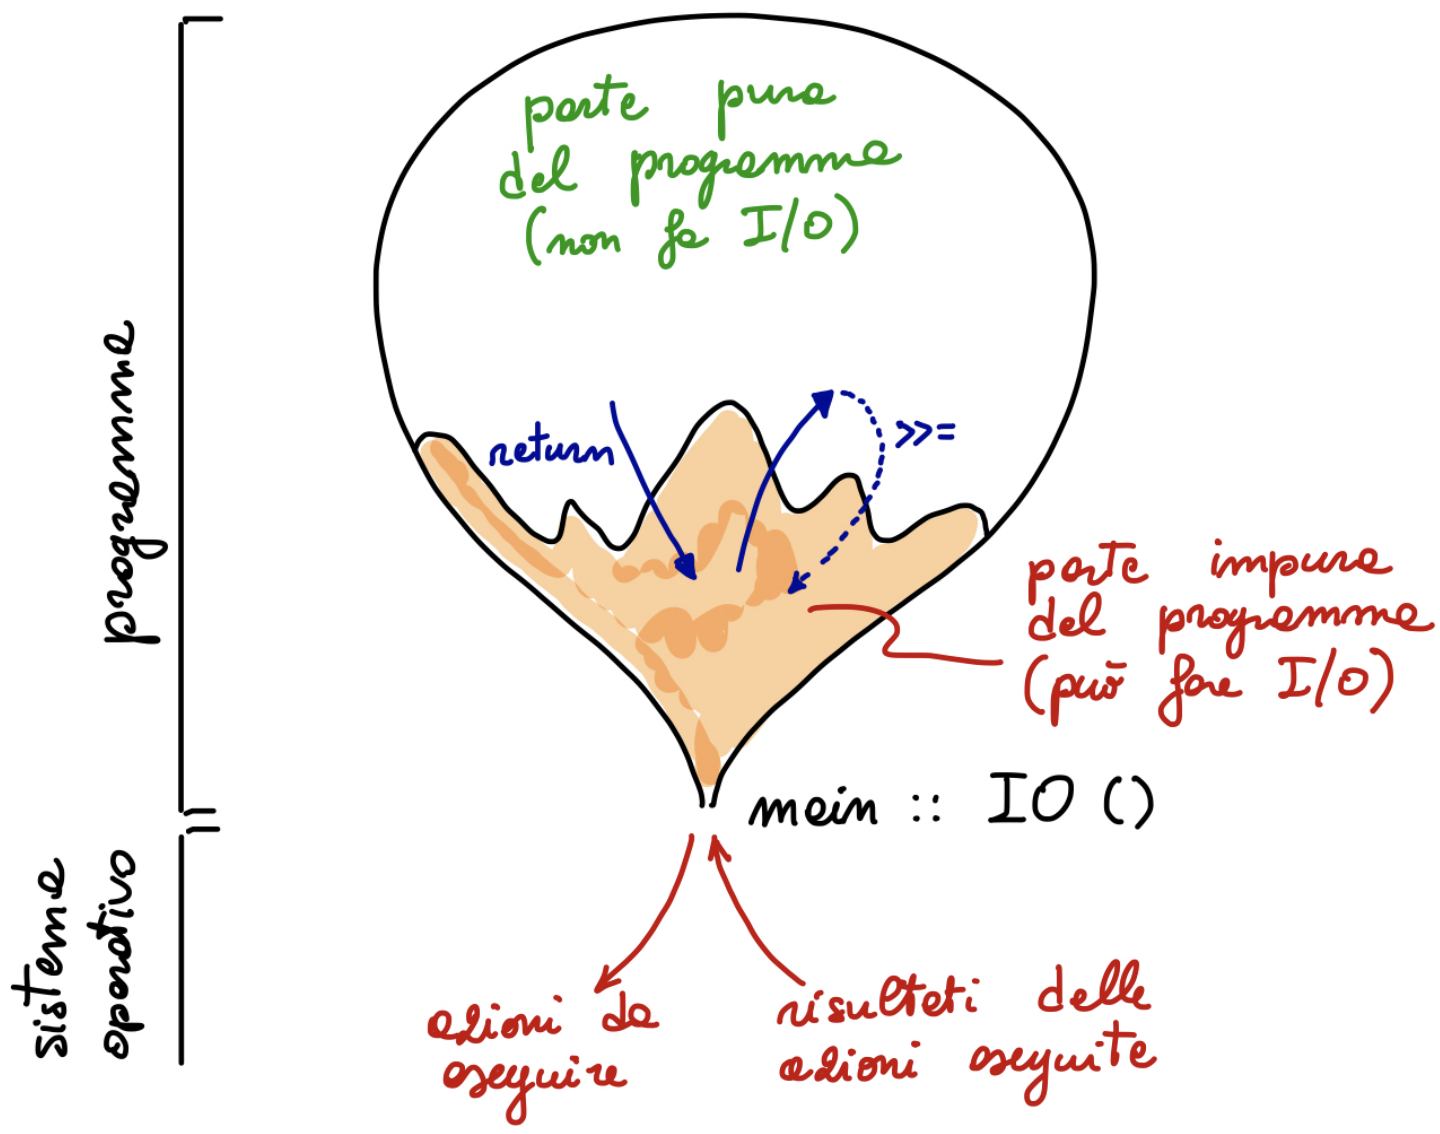
\includegraphics[width=0.8\textwidth]{img/monadi.png}
\end{center}

E' quindi presente una suddivisione tra la parte \textit{pura} e \textit{impura} del programma. Il nostro programma rimane puro, delegando al sistema operativo l'esecuzione di funzionalità impure.

Inizialmente l'idea delle monadi era stata pensata per gestire il problema dell'input/output. Successivamente ci si è resi conto che poteva essere utilizzata anche per altri scopi (alcuni possono essere eccezioni, parallelismo, transazioni).

Una monade può essere anche definita come: concetto nell’area della semantica dei linguaggi per descrivere matematicamente \textbf{computazioni} che possono avere \textbf{effetti collaterali}.

E' possibile trovare monadi anche in linguaggi moderni, come Scala e Javascript, fornendo un modo strutturato di organizzare computazioni con effetti collaterali.\vspace{14pt}\\
Di seguito vengono mostrati esempi pratici di applicazione di monadi in Haskell.

\pagebreak

\subsection*{Valutatore di espressioni}
Si vuole realizzare un valutatore per semplici espressioni aritmetiche.
\begin{tcolorbox}
\begin{verbatim}
data Expr = Const Int | Div Expr Expr

eval :: Expr -> Int
eval (Const n) = n
eval (Div t s) = eval t ‘div‘ eval s
\end{verbatim}
\end{tcolorbox}
\texttt{Expr} indica una struttura dati custom, la quale può avere un valore \texttt{Int} oppure rappresentare una espressione aritmetica.

Vengono successivamente definiti due casi possibili: restituzione del valore inviato e calcolo dell'espressione.

Si vuole ora raffinare il valutatore in modo che supporti:
\begin{itemize}
    \item Gestione delle \textbf{divisioni per zero}
    \item \textbf{Conteggio} delle operazioni “difficili”
    \item \textbf{Tracciamento} dei passi di valutazione
\end{itemize}
Se usassimo un linguaggio impuro sarebbe tutto facile.\vspace{14pt}\\
Partiamo dalla divisione per zero.\\
Per implementare la gestione della divisione per zero viene modificato il codice nel seguente modo:
\begin{tcolorbox}
\begin{verbatim}
eval :: Expr -> Maybe Int
eval (Const n) = Just n
eval (Div t s) =
    case eval t of
        Nothing -> Nothing
        Just m -> case eval s of
            Nothing -> Nothing
            Just 0 -> Nothing
            Just n -> Just (m ‘div‘ n)
\end{verbatim}
\end{tcolorbox}
Ciò che era facile fare in un linguaggio impuro ha stravolto la struttura del programma in un linguaggio puro. La logica del programma si perde nella gestione dell’eccezione.

\pagebreak

Si passa ora al conteggio delle operazioni "difficili".\\
Per implementare il conteggio delle operazioni viene modificato il codice nel seguente modo:
\begin{tcolorbox}
\begin{verbatim}
type Counter a = Int -> (a, Int)

eval :: Expr -> Counter Int
eval (Const n) x = (n, x)
eval (Div t s) x =
    let (m, y) = eval t x in
        let (n, z) = eval s y in
            (m ‘div‘ n, z + 1)
\end{verbatim}
\end{tcolorbox}
Ciò che era facile fare in un linguaggio impuro ha stravolto la struttura del programma in un linguaggio puro. La logica del programma si perde nella gestione del contatore.\vspace{14pt}\\
Per concludere, si passa al tracciamento dei passi di valutazione.\\
Per implementare il tracciamento dei passi di valutazione viene modificato il codice nel seguente modo:
\begin{tcolorbox}
\begin{verbatim}
type Output a = (String, a)

eval :: Expr -> Output Int
eval (Const n) = (line (Const n) n, n)
eval (Div t s) =
    let (x, m) = eval t in
        let (y, n) = eval s in
            (x ++ y ++ line (Div t s) (m ‘div‘ n), m ‘div‘ n)

line :: Expr -> Int -> String
line t n = "eval (" ++ show t ++ ") = " ++ show n ++ "\n"
\end{verbatim}
\end{tcolorbox}
Ciò che era facile fare in un linguaggio impuro ha stravolto la struttura del programma in un linguaggio puro. La logica del programma si perde nella gestione della traccia.

In tutti e tre i casi, l'utilizzo di un linguaggio puro porta ad un codice più complesso.\vspace{14pt}\\
Si vuole ora fare una sorta di esercizio di astrazione.

Prendendo una versione \textbf{pura} di \texttt{eval}, si ha \texttt{\quad eval :: Expr -> Int}

Prendo una versione \textbf{impura} di \texttt{eval}, si ha \texttt{\quad eval :: Expr -> M Int}\\
dove \texttt{M} può essere:
\begin{itemize}
    \item \textbf{Maybe}, nel caso delle eccezioni
    \item \textbf{Counter}, nel caso del contatore
    \item \textbf{Output}, nel caso del tracciamento
\end{itemize}
Su queste \texttt{M} occorrono diverse operazioni specifiche che dipendono dalla \texttt{M} stessa. Sono però sempre presenti due operazioni:
\begin{itemize}
    \item \textbf{return}: l'idea dietro la funzione \texttt{return} è che la sua computazione debba essere pura, senza effetti collaterali. Viene definita come 
    \begin{center}
        \texttt{return :: a -> M a}
    \end{center}
    \item \textbf{bind ($>>=$)}: l'idea dietro la funzione \texttt{bind} è il combinare in sequenza due computazioni della monade \texttt{M}, dove però la seconda computazione può aver bisogno di conoscere il valore prodotto dalla computazione precedente. Viene definita come
    \begin{center}
        \texttt{$(>>=)$ :: M a -> (a -> M b) -> M b }    
    \end{center}
\end{itemize}
Questi due sono gli operatori fondamentali di ogni monade, che ci permettono di dire come viene fatta una computazione pura e come vengono combinate in sequenza più operazioni.

Oltre a queste due, ogni monade avrà delle operazioni ad hoc per gestire i casi specifici inerenti.

Tornando all'esempio precedente, osserviamo ora come implementare le monadi in quel contesto, andando a semplificare il codice.\vspace{14pt}\\
Partiamo dalla divisione per zero. Il codice in versione monadica è il seguente:
\begin{tcolorbox}
\begin{verbatim}
return :: a -> Maybe a
return = Just

(>>=) :: Maybe a -> (a -> Maybe b) -> Maybe b
(>>=) Nothing _ = Nothing
(>>=) (Just a) f = f a

abort :: Maybe a
abort = Nothing

evalM :: Expr -> Maybe Int
evalM (Const n) = return n
evalM (Div t s) =
    evalM t >>= \m ->
    evalM s >>= \n ->
    if n == 0 then abort
    else return (m ‘div‘ n)
\end{verbatim}
\end{tcolorbox}
In questo caso, la funzione \texttt{return} viene scritta in maniera abbreviata. La sua forma completa è \texttt{return a = Just a}. Questa funzione ci permette di indicare la computazione pura andando ad affermare che dato un argomento \texttt{a}, la funzione \texttt{return} restituirà semplicemente un valore \texttt{Just a}.

Per quanto riguarda la funzione \texttt{bind} sono presenti due casi.

Nel primo caso viene gestito il fallimento, con \texttt{Nothing} come parametro di sinistra che restituisce un ulteriore valore \texttt{Nothing} per indicare il fallimento della composizione di operazioni.

Nel secondo caso, invece, la prima computazione è andata a buon fine e sarà quindi possibile applicare \texttt{f} ad \texttt{a} (tramite \texttt{f a}).

E' inoltre presente una operazione specifica chiamata \texttt{abort}, la quale permette di restituire un \texttt{Nothing} abortendo la computazione.

Grazie a queste nuove funzioni, si può riscrivere il codice in maniera più ordinata e leggibile.\vspace{14pt}\\
Si passa ora al conteggio delle operazioni "difficili". Il codice in versione monadica è il seguente:
\begin{tcolorbox}
\begin{verbatim}
return :: a -> Counter a
return a = \x -> (a, x)

(>>=) :: Counter a -> (a -> Counter b) -> Counter b
(>>=) m f = \x -> let (a, y) = m x in f a y

tick :: Counter ()
tick = \x -> ((), x + 1)

evalM :: Expr -> Counter Int
evalM (Const n) = return n
evalM (Div t s) =
    evalM t >>= \m ->
    evalM s >>= \n ->
    tick >>= \() ->
    return (m ‘div‘ n)
\end{verbatim}
\end{tcolorbox}
In questo caso, la funzione \texttt{return} può esprimere una computazione pura solo nel caso in cui non viene modificato il contatore. Viene quindi passato l'argomento \texttt{x} senza essere alterato.

Per quanto riguarda la funzione \texttt{bind}, il valore del contatore \texttt{x} viene passato ad \texttt{m} per essere alterato. Il valore modificato \texttt{y} rappresenterà il nuovo valore del contatore. Il contatore viene quindi passato dalla prima computazione alla successiva, per essere alterato.

E’ inoltre presente una operazione specifica chiamata \texttt{tick}, la quale permette di incrementare il valore del contatore di uno. Le parentesi tonde aperte chiuse indicano una \texttt{Unit}, un valore vuoto.

Grazie a queste nuove funzioni, si può riscrivere il codice in maniera più ordinata e leggibile.

Si può anche notare come i due codici appena presentati risultano essere simili nella loro forma, anche se gli effetti collaterali causati dalle monadi sono differenti.

\pagebreak

Per concludere, si passa al tracciamento dei passi di valutazione. Il codice in versione monadica è il seguente:
\begin{tcolorbox}
\begin{verbatim}
return :: a -> Output a
return a = ("", a)

(>>=) :: Output a -> (a -> Output b) -> Output b
(>>=) m f =
  let (x, a) = m in
    let (y, b) = f a in
      (x ++ y, b)

output :: String -> Output ()
output x = (x, ())

evalM :: Expr -> Output Int
evalM (Const n) =
  output (line (Const n) n) >>= \() ->
  return n
evalM (Div t s) =
  evalM t >>= \m ->
  evalM s >>= \n ->
  output (line (Div t s) (m `div` n)) >>= \() -> return (m `div` n)
\end{verbatim}
\end{tcolorbox}
Anche in questo caso , come per i precedenti, le funzioni \texttt{return} e \texttt{bind} permettono di esprimere la computazione pura e la composizione di operazioni.

Per quanto riguarda le operazioni speciali, è presente la funzione \texttt{output}, la quale permette di ottenere una traccia a schermo.\vspace{14pt}\\
Volendo ricapitolare i casi appena visti, si può effettuare la seguente suddivisione di monadi:
\begin{itemize}
    \item \textbf{Maybe a}: per le computazioni che possono fallire (con \texttt{abort}). Se hanno successo producono un valore di tipo \texttt{a}.
    \item \textbf{Counter a}: per le computazioni che possono incrementare un contatore (con \texttt{tick}). Producono un valore di tipo \texttt{a}.
    \item \textbf{Output a}: per le computazioni che possono produrre una traccia (con \texttt{output}). Producono un valore di tipo \texttt{a}.
\end{itemize}

\pagebreak

Si vuole ora dare una definizione di \textbf{monade}.

Il termine monade deriva da \textit{monoide}, ovvero una struttura algebrica dotata di un'operazione \textbf{assiociativa}:
\begin{center}
    \texttt{(a * b) * c = a * (b * c)}
\end{center}
e con unità (o elemento neutro) \texttt{e} a sinistra e destra:
\begin{center}
    \texttt{a * e = e * a = a}
\end{center}

Se leggiamo \texttt{*} come composizione ed \texttt{e} come nessun effetto, queste proprietà di un monoide dicono che:
\begin{itemize}
    \item Non c’è differenza tra comporre \texttt{c} con la composizione di \texttt{a} e \texttt{b} e comporre \texttt{a} con la composizione di \texttt{b} e \texttt{c}, purché l’ordine delle azioni sia preservato (un monoide \textbf{non è} commutativo in generale).
    \item La neutralità di \texttt{e} cattura il fatto che esso rappresenti una azione “pura”, priva di effetti.
\end{itemize}
\vspace{8pt}
Una monade non è propriamente un monoide perché c'è bisogno di trasferire informazioni tra le computazioni combinate.

Per questo motivo vengono formulate \textbf{tre leggi} per rappresentare una monade, che sono:
\begin{enumerate}
    \item \quad \texttt{return a $>>=$ f $\equiv$ f a}
    \item \quad \texttt{m $>>=$ return $\equiv$ m}
    \item \quad \texttt{(m $>>=$ $\backslash a$ -> n) $>>=$ f $\equiv$ m $>>=$ ($\backslash a$ -> n $>>=$ f)}
\end{enumerate}
Le prime due leggi affermano che \texttt{return} si comporta come un elemento neutro (computazione pura, priva di effetti).

La terza legge afferma che \texttt{bind} è associativo (N.B.: solo se \texttt{a} non compare libera in \texttt{f}).

Queste leggi vanno \textbf{dimostrate} per ogni monade.\vspace{14pt}\\
Si vuole ora provare a dimostrare le tre leggi per la monade \texttt{Maybe}. Riprendendo la sua definizione di \texttt{return} e \texttt{bind}:
\begin{tcolorbox}
\begin{verbatim}
return :: a -> Maybe a
return = Just

(>>=) :: Maybe a -> (a -> Maybe b) -> Maybe b
(>>=) Nothing _ = Nothing
(>>=) (Just a) f = f a
\end{verbatim}
\end{tcolorbox}
Partendo dalla prima legge, si può dimostrare con:
\begin{center}
    \texttt{return a $>>=$ f \qquad=\qquad Just a $>>=$ f \qquad=\qquad f a}
\end{center}
Passando invece alla seconda legge, vanno dimostrati due casi possibili:
\begin{center}
    Caso \texttt{m = Nothing}:\\
    \texttt{m $>>=$ return \qquad=\qquad Nothing \qquad=\qquad m}\\
    Caso \texttt{m = Just a}:\\
    \texttt{m $>>=$ return \qquad=\qquad return a \qquad=\qquad Just a \qquad=\qquad m}
\end{center}
Per concludere con la terze legge, che dimostra l'associatività, vanno dimostrati il lato sinistro e destro dei due casi possibili:
\begin{center}
    Lato sinistro, Caso \texttt{m = Nothing}:\\
    \texttt{(m $>>=$ $\backslash$a -> n) $>>=$ f \qquad=\qquad (Nothing $>>=$ $\backslash$a -> n) $>>=$ f \\ \qquad=\qquad Nothing $>>=$ f \qquad=\qquad Nothing}\vspace{10pt}\\
    Lato sinistro, Caso \texttt{m = Just a}:\\
    \texttt{(m $>>=$ $\backslash$a -> n) $>>=$ f \qquad=\qquad (Just a $>>=$ $\backslash$a -> n) $>>=$ f \\ \qquad=\qquad (($\backslash$a -> n) a) $>>=$ f \qquad=\qquad n $>>=$ f}\vspace{14pt}\\
    Lato destro, Caso \texttt{m = Nothing}:\\
    \texttt{m $>>=$ ($\backslash$a -> n $>>=$ f) \qquad=\qquad Nothing $>>=$ ($\backslash$a -> n $>>=$ f) \\ \qquad=\qquad Nothing}\vspace{10pt}\\
    Lato destro, Caso \texttt{m = Just a}:\\
    \texttt{m $>>=$ ($\backslash$a -> n $>>=$ f) \qquad=\qquad Just a $>>=$ ($\backslash$a -> n $>>=$ f) \\ \qquad=\qquad ($\backslash$a -> n $>>=$ f) a \qquad=\qquad n $>>=$ f}
\end{center}
\vspace{8pt}
Avendo dimostrato le tre leggi, \texttt{Maybe} viene considerata una monade.

Discorso analogo può essere fatto anche per \texttt{Counter} e \texttt{Output} (dimostrazioni sulle slide).\vspace{14pt}\\
Viene ora fatta un'osservazione: \texttt{return} e \texttt{bind} sono \textbf{overloaded} (dipendono dalla singola monade).

L'idea di base è la definizione di una classe di \textbf{costruttori di tipo} \texttt{Monad}:
\begin{tcolorbox}
\begin{verbatim}
class Monad m where
    return :: a -> m a
    (>>=) :: m a -> (a -> m b) -> m b
\end{verbatim}
\end{tcolorbox}
dove \texttt{m} è una variabile su \textbf{costruttori di tipo}.\vspace{14pt}\\
Un ulteriore concetto utile quando si programma con le monadi è la funzione \textbf{and then $>>$}.

A volte quando si combinano due azioni di una monade, la seconda non usa il risultato della prima e solo la composizione degli effetti è importante.

Una possibile definizione di questa funzione, che si può generalizzare ad ogni monade, può essere:
\begin{tcolorbox}
\begin{verbatim}
(>>) :: Counter a -> Counter b -> Counter b
(>>) as bs = as >>= const bs
\end{verbatim}
\end{tcolorbox}

\pagebreak

Un suo possibile esempio di utilizzo, nel contesto precedentemente visto di Counter, può essere:
\begin{tcolorbox}
\begin{verbatim}
evalN :: Expr -> Counter Int
evalN (Const n) = return n
evalN (Div t s) =
    evalN t >>= \m ->
    evalN s >>= \n ->
    tick >>
    return (m ‘div‘ n)
\end{verbatim}
\end{tcolorbox}
dove la riga \texttt{tick $>>=$ $\backslash$()} diventa solamente \texttt{tick $>>$}.\vspace{14pt}\\
Un altro concetto, principalmente zucchero sintattico, è quello della notazione \textbf{do}. Riprendendo un esempio visto in precedenza:
\begin{tcolorbox}
\begin{verbatim}
evalM :: Expr -> Maybe Int
evalM (Const n) = return n
evalM (Div t s) =
    evalM t >>= \m ->
    evalM s >>= \n ->
    if n == 0 then abort
    else return (m ‘div‘ n)
\end{verbatim}
\end{tcolorbox}
Attraverso la notazione \texttt{do} si può semplificare in:
\begin{tcolorbox}
\begin{verbatim}
evalM :: Expr -> Maybe Int
evalM (Const n) = return n
evalM (Div t s) = do
    m <- evalM t
    n <- evalM s
    if n == 0 then abort
    else return (m ‘div‘ n)
\end{verbatim}
\end{tcolorbox}
\vspace{14pt}
Si osserva ora la possibilità di avere una monade che rappresenta computazioni con effetti molteplici di natura diversa. Questo approccio non è immediato e presenta alcune problematiche.

Il primo problema è di natura concettuale. E' infatti presenta un'ambiguità semantica. Osserviamo due esempi di semantiche differenti:
\begin{itemize}
    \item Semantica \textit{tradizionale}: \texttt{eval :: Expr -> Int -> (Maybe Int, Int)}
    \item Semantica \textit{transazionale}: \texttt{eval :: Expr -> Int -> Maybe (Int, Int)}
\end{itemize}
A seconda di quale semantica si sceglie, si va a cambiare il significato della valutazione.

Nella prima semantica, il contatore viene incrementato anche in caso di fallimento dell'ultima valutazione.

Nella seconda, invece, in caso di fallimento dell'ultima valutazione si ottiene un \texttt{Nothing}, perdendo il valore del contatore. Si applica una logica transazionale, come nei database.\vspace{14pt}\\
Il secondo problema è di natura ingegneristica. Creando una singola monade che combina più effetti si crea il problema del dover duplicare il codice.\vspace{14pt}\\
Questi due problemi, con l'idea di monade osservata fino ad ora, non ci permettono di ottenere più effetti con una singola monade.

Si introduce quindi una nuova idea: invece di definire una monade per rappresentare computazioni che possono avere “certi effetti”, definiamo una \textbf{trasformazione di monade} che \textbf{aggiunge} “certi effetti” a una monade già esistente.

Si osservi una possibile trasformazione \texttt{MaybeT} (N.B.: il codice visto d'ora in poi è corretto in forma logica, ma viene rifiutato dal compilatore Haskell. Per risolvere questo problema si dovrebbero usare i tipi inversi delle monadi):
\begin{tcolorbox}
\begin{verbatim}
type MaybeT m a = m (Maybe a)

instance Monad m => Monad (MaybeT m) where
    return = return . Just
    (>>=) m f = m >>= \x ->
        case x of
            Nothing -> return Nothing
            Just a -> f a

abort :: Monad m => MaybeT m a
abort = return Nothing
\end{verbatim}
\end{tcolorbox}
Partendo dalla definizione di \texttt{return}, volendo riscriverla in forma estesa: \\ \texttt{return a = return (Just a)} . Il \texttt{return} esterno fa riferimento alla funzione della monade \texttt{MaybeT}, mentre quello interno fa riferimento alla monade \texttt{m}.

Passando invece alla definizione di \texttt{bind}, vale lo stesso discorso fatto in precedenza per \texttt{return}. Le funzioni di \texttt{bind} esterna ed interna fanno riferimento a due funzioni diverse.

\pagebreak

Volendo quindi applicare la monade \texttt{MaybeT} ad un esempio concreto:
\begin{tcolorbox}
\begin{verbatim}
type MaybeCounter = MaybeT Counter

evalM :: Expr -> MaybeCounter Int
evalM (Const n) = return n
evalM (Div t s) =
    evalM t >>= \m ->
    evalM s >>= \n ->
    tick >>= \() ->         -- ERRORE!
    if n == 0 then abort
    else return (m ‘div‘ n)
\end{verbatim}
\end{tcolorbox}
Non possono essere mescolate azioni di monadi diverse. \texttt{tick} fa parte della monade interna, ma non può essere richiamata in questo modo.

Per risolvere questo problema si introduce il concetto di \textbf{lifting delle operazioni}.

Quando usiamo \texttt{MaybeT} per trasformare una monade \texttt{m} in una monade \texttt{MaybeT m}, vorremmo poter trasformare computazioni di \texttt{m} (che non possono fallire) in computazioni di \texttt{MaybeT m} che non falliscono.

Questa trasformazione di computazioni si chiama \textbf{lifting}. Ogni trasformazione di monade avrà il suo lifting specifico, per cui ha senso definire una classe con una funzione \texttt{lift}.
\begin{tcolorbox}
\begin{verbatim}
class MonadT t where
    lift :: Monad m => m a -> t m a
\end{verbatim}
\end{tcolorbox}
\vspace{8pt}
Riprendendo l'esempio di \texttt{MaybeT}:
\begin{tcolorbox}
\begin{verbatim}
instance MonadT MaybeT where
    lift m = m >>= (return . Just)
\end{verbatim}
\end{tcolorbox}
con conseguente codice funzionante:
\begin{tcolorbox}
\begin{verbatim}
evalM :: Expr -> MaybeCounter Int
evalM (Const n) = return n
evalM (Div t s) =
    evalM t >>= \m ->
    evalM s >>= \n ->
    lift tick >>= \() ->    -- OK!
    if n == 0 then abort
    else return (m ‘div‘ n)
\end{verbatim}
\end{tcolorbox}

\pagebreak

Con \texttt{MaybeT} possiamo aggiungere fallimenti a qualsiasi monade, inclusa \texttt{Counter}. 

Se definiamo la trasformazione di monade \texttt{CounterT} possiamo aggiungere un contatore a qualsiasi monade, inclusa \texttt{Maybe}.

Questo porta ad avere un totale di 2 trasformazioni di monadi + 2 monadi.

Se definiamo una monade \textit{banale} \textbf{Id} per rappresentare computazioni pure (prive di effetti), possiamo ottenere ogni combinazione come pila di trasformazioni che partono da Id.

Degli esempi possono essere \texttt{Maybe = MaybeT Id} e \texttt{Counter = CounterT Id}.

Una definizione di \texttt{Id} può essere:
\begin{tcolorbox}
\begin{verbatim}
type Id a = a

instance Monad Id where
    return = id
    (>>=) a f = f a
\end{verbatim}
\end{tcolorbox}
\vspace{8pt}
Volendo applicare questo concetto su \texttt{CounterT} (N.B.: anche questo codice non viene accettato dal compilatore Haskell, ma resta logicamente corretto):
\begin{tcolorbox}
\begin{verbatim}
type CounterT m a = Int -> m (a, Int)

instance Monad m => Monad (CounterT m) where
    return a = \x -> return (a, x)
    (>>=) m f = \x -> m x >>= \(a, y) -> f a y

tick :: Monad m => CounterT m ()
tick = \x -> return ((), x + 1)
\end{verbatim}
\end{tcolorbox}
\end{document}